\documentclass[tikz,border=5]{standalone}
\usepackage{tikz}
\usetikzlibrary{circuits.ee.IEC}

\usepackage{amsmath, amssymb}

%CIRCUIT SYMBOL converter %%%%%%%%%%%%%%%%%
\tikzset{circuit declare symbol = converter}
\tikzset{set converter graphic = converter IEC graphic}
\tikzset{convert from/.initial=AC,
         convert from/.default=AC,
         convert to/.initial=DC,
         convert to/.default=DC}
\tikzset{converter IEC graphic/.style=
  {transform shape, circuit symbol lines, circuit symbol size = width
2.5 height 2.5, draw=none, rounded corners=2.25pt,
   shape=generic circle IEC, /pgf/generic circle IEC/before
background=
    {
     %CROSSLINE
     \pgfpathmoveto{\pgfpoint{-0.8pt}{-0.8pt}}
     \pgfpathlineto{\pgfpoint{0.8pt}{0.8pt}}
     %RECTANGLE
     \pgfpathrectangle{\pgfpoint{-1pt}{-1pt}}{\pgfpoint{2.0pt}{2.0pt}}
     \pgfusepath{stroke} 
     \pgfusepathqstroke
     % TEXT INSIDE THE SYMBOL
     \pgfgettransform\savedtransform
     \pgftransformshift{\pgfpoint{0.45pt}{-0.45pt}}
     \pgftransformresetnontranslations
     \pgftransformscale{0.075\tikzcircuitssizeunit}
     \pgftext{\bf{\pgfkeysvalueof{/tikz/convert to}}}
     \pgfsettransform\savedtransform
     \pgftransformshift{\pgfpoint{-0.45pt}{0.45pt}}
     \pgftransformresetnontranslations
     \pgftransformscale{0.075\tikzcircuitssizeunit}
     \pgftext{\bf{\pgfkeysvalueof{/tikz/convert from}}}
     \pgfsettransform\savedtransform
     }}}
%%%%%%%%%%%%%%%%%%%%%%%%%%%%%%%

%===========
\begin{document}
%===========

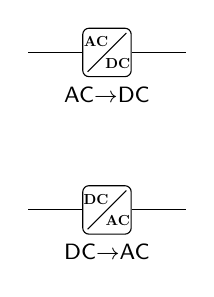
\begin{tikzpicture}[circuit ee IEC, font=\sffamily\footnotesize]
    % First converter (AC -> DC)
    \draw (0,0) to [converter={info'={AC$\rightarrow$DC},
      convert from={AC}, convert to={DC}}] (2,0);
      
    % Second converter (DC -> AC) positioned to the right
    \draw (0,-2) to [converter={info'={DC$\rightarrow$AC},
      convert from={DC}, convert to={AC}}] (2,-2);

\end{tikzpicture}

%===========
\end{document}
%===========
